\documentclass[11pt,a4paper]{report}
\usepackage[cp1250]{inputenc}
\usepackage[english]{babel}
\usepackage[IL2]{fontenc}
\usepackage{amsmath}
\usepackage{amsfonts}
\usepackage{amssymb}
\usepackage{makeidx}
\usepackage{graphicx}
\usepackage{lmodern}
\usepackage{subfig}
\usepackage[autostyle]{csquotes}
\usepackage{setspace}
\usepackage[
backend=bibtex        % if we want unicode
,style=iso-authoryear % or iso-numeric for numeric citation method
,autolang=other       % to support multiple languages in bibliography      
]{biblatex}
\usepackage{multicol}
\usepackage{titlesec}    
\titleformat{\chapter}[block]
{\normalfont\Large\bfseries}{\thechapter.}{1em}{\Large}
\titlespacing*{\chapter}{0pt}{-19pt}{19pt}


\titleformat{\section}[block]
{\normalfont\large\bfseries}{\thesection.}{1em}{\large}
\titlespacing*{\section}{0pt}{11pt}{19pt}


\usepackage{scrpage2}
\ifoot[]{}
\cfoot[]{}
\ofoot[\pagemark]{\pagemark}


\newcommand{\fakeparagraph}[1]{%
	\par\refstepcounter{paragraph}% Increase paragraph counter
	\paragraphmark{#1}% Add paragraph mark (header)
}



\graphicspath{ {./images/} }

\makeatletter
\def\blx@maxline{77}
\makeatother

\bibliography{Thesis.bib}

\newcommand*{\captionsource}[2]{%
	\caption[{#1}]{%
		#1%
		\\\hspace{\linewidth}%
		\textbf{Source:} #2%
	}%
}

\pagenumbering{gobble}

\usepackage[left=3.5cm,right=2cm,top=2cm,bottom=2cm]{geometry}
\author{Bc. Michal Koh�tek}
\title{Rozpozn�vanie emocion�lneho stavu pou��vate�a pomocou inteligentn�ch 
riadiacich syst�mov}
\begin{document}
	
\begin{titlepage}
	
{\centering
{\bfseries\LARGE UNIVERZITA KON�TANT�NA FILOZOFA V NITRE \par}
{\bfseries\LARGE FAKULTA PR�RODN�CH VIED \par}
\vfill
{\bfseries\LARGE ROZPOZN�VANIE EMOCION�LNEHO STAVU POU��VATE�A POMOCOU 
INTELIGENTN�CH RIADIACICH SYST�MOV\par}
\vspace{1cm}
{\bfseries\Large Diplomov� pr�ca\par}
\par}
\vfill
\Large{
�tudijn� program: Aplikovan� informatika (magistersk� II. St., denn�  
forma)\par
�tudijn� odbor:  AI15m - Aplikovan� informatika\par
�koliace pracovisko: Katedra Matematiky\par
�kolite�: Mgr. Martin Magdin, PhD\par}
\vfill
\textbf{Nitra 2018}\hfill\textbf{Bc. Michal Koh�tek}
\end{titlepage}
\onehalfspacing
\chapter*{Abstrakt}

\chapter*{Abstract}


Abstract goes here

\chapter*{Dedication}
To mum and dad

\chapter*{Declaration}
I declare that..

\chapter*{Acknowledgements}
I want to thank...

\tableofcontents
 
\chapter*{Introduction}
\pagenumbering{arabic}
\setcounter{page}{8}
\pagestyle{scrplain}
\begin{flushright}

"Smiles are probably the most underrated \\ facial expressions, 
 much more complicated \\ than most people realize. 
 There are dozens\\ of smiles, each differing in appearance \\
 and in the message expressed."\\
 - Paul Ekman
\end{flushright}

\paragraph{} Emotions are at the core of the human experience, albeit very hard 
to define, recognize and name, even in yourself. They are, by definition 
different from person to person, in diverse cultures and upbringings. Our 
perception of emotions and their classification has evolved in recent years. 
Various authors has tried to divide our emotional states into basic categories 
such as Ekman's Anger, Fear, Disgust, Happiness, Sadness and Surprise. However, 
recent work by psychologists and historians alike show, that a more complex 
look at emotions might be needed. 

\paragraph{}Emotional recognition changes with time. In 12th century, bards 
looked at yawning not as a sign of boredom or tiredness, but as a sign of a 
hidden and deep love. Early Christians recognized an emotion called "accidie", 
a lethargy and despair brought about by flying demons. Boredom, as such was 
first really  felt by the Victorians as a response to the new ideas of leisure 
time and self-improvement. Among the psychologist, there is a standing question 
whether some cultures feel some hard to define emotions more strongly, because 
they bothered to name them as separate kinds. For example the Russian "toska", 
a longing with nothing to long for, as coined by Vladimir Nabokov. Recent 
developments of cognitive science tell us, that emotions are not just simple 
reflexes, but inherently complex and elastic systems of response towards both 
the biologies 
that we've inherited and the cultures, that we live in now. They are not just 
simple chemistry, but a cognitive phenomena, not shaped only by our body 
functions, but also our thought process, concepts and language. The 
neuroscientist Lisa Feldman Barrett studies this 
dynamic relationship between words and emotions. She argues, that when a person 
learns a new word for an emotion, they also learn to feel and recognize it 
(\cite{barrett}). 
There is a historicity to emotions, they have changed in history, often times 
very dramatically, in response to new cultural expectations, religious beliefs, 
new ideas about gender, age, ethnicity, economical and political ideologies. 

\paragraph{}There is a push to increase our emotional intelligence. Emotions 
are so 
powerful, that in past, they were sometimes thought to be a cause of illness. 
In 17th century, there was a student attending the Swiss university in Basel. 
He 
came afflicted with fever, heart palpitations, skin sores on his body and was 
close to dying. When they sent him back home to die, he started getting better 
and by the time, he returned to his hometown, he almost entirely recovered. In 
1688, Johannes Hoffer, medical doctor, learnt of this case and 
many like it and coined the term for a severe homesickness as "nostalgia". Last 
confirmed death by nostalgia was an American soldier fighting during the First 
World War in France. In early 20th century, this feeling has morphed more into 
a longing for lost time, instead of homesickness and downgraded in severity. 
Nowadays, our culture celebrates happiness, as it is said to make 
us a better workers, parents and partners. However, in 16th century, this 
position was filled by sadness, as is evident by self-help books from that 
period, which tried to encourage sadness in readers by giving them lists of 
reasons to be disappointed.

\paragraph{}In order to study both basic emotions and their mixtures in the 
complex variety, we need appropriate detection and classification tools and 
techniques. Over the years, many psychologists and computer scientist 
collaborated to create a set of markers and techniques recognizing them. We 
will discuss several of them and compare their usefulness, reliability and 
practicality. These methods most often try to detect basic emotions such as the 
seven basic emotions (\cite{Ekman}) or a 12-point Affect Circumplex model 
(\cite{Russel}).
\begin{figure} [ht]
	\centering
	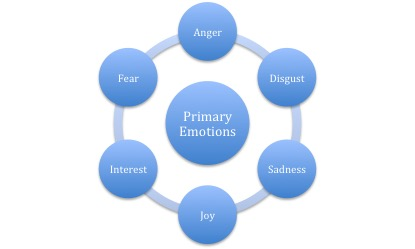
\includegraphics[scale=0.6]{images/Primary_Emotions}
	\caption{Six primary emotions}
	\label{fig:}
\end{figure} 

\paragraph{}Affective computing has great many possible applications. It can 
allow for a better education process, providing a large amount of valid 
feedback to the tutors and students (\cite{Asteriadis2008EstimationOB}). It can 
help broaden the knowledge in the study of psychology and psychiatry, improve 
the efficiency of counseling. Since emotions recognition and empathy is one of 
the traits of inter-personal communication, properly analyzing emotions can 
help in developing communicative technologies for use by people with autism. 
Growing interest in affective computing is shown by many industries. Automobile 
manufacturers are partnering with companies like Affectiva and integrating 
their solutions in their high-end cars (\cite{affectiva}). Other venue for 
emotion recognition is targeted marketing. In past, online e-commerce sites 
would often use "heat maps" to see, whether the potential customer can find 
products on the website, and whether the paid advertisement holds their 
attention. If the same system added emotion recognition, online marketers would 
gain greater insight into minds of customers. Another future purpose for 
affective computing may be found in robotic pets and social robots, especially 
those working in health 
care industry. Emotional awareness could allow robotic nurses to better judge 
users' and patient's emotional states and needs (\cite{yonck2017heart}). It is 
clear, that affective computing will grow to become an important aspect of 
computer science theory.




\chapter{Emotion classification} \paragraph{}Emotion classification is a 
contested issue in 
emotion research and in affective science. The two fundamental viewpoints of 
affective scientists' approach are: \begin{enumerate}
	\item Emotions as discrete and fundamentally different constructs
	\item Emotions as fluid and characterized on a dimensional basis in 
	groupings
\end{enumerate}
Various categorizations of emotions also vary in description how emotions 
relate to each other.
\section{Discrete models of emotions}
\paragraph{}Discrete emotion theory claims that there is a small 
number 
of core affects. 
This number can vary depending on the proponent, for example Silvan Tomkins 
considered nine basic emotions. Six, that came evolutionarily earlier, 
interest-excitement, enjoyment-joy, surprise-startle, distress-anguish, 
anger-rage, fear-terror, once that evolved later, shame-humiliation and finally 
disgust and dissmell, which he later took back. In the paired affects, the 
first of the pair is the mild manifestation and the second the more intense. 
(\cite{tomkins1962affect}), (\cite{tomkins1963affect}). This model is somewhat 
controversial nowadays among affective theorists, especially over Tomkins' firm 
insistence that there were nine and only nine, biologically based affects. He 
also argued, that these affects are quite discreet (in contrast to the more 
muddled and complex emotions) and that they shared a common biological heritage 
with what Darwin called emotions in animals (\cite{darwin1998expression}). They 
also differ from Freudian drives in lacking an object.
\paragraph{}Similarly, Carroll Izard delineated 12 discrete emotions: 
interest, joy, surprise, sadness, anger, disgust, contempt, self-hostility, 
fear, shame, shyness and guild. He measured these via his Differential Emotion 
Scale (\cite{Izard}). Among other contributors to this theory, such as John 
Watson, Edwin Newman and Ross Buck, Paul Ekman performed a series of 
cross-cultural studies with Carrol Izard and reported that there are at least 
six emotions, that people across the world produce and are able to recognize. 
This was further evidenced when researchers approached the people of New Guinea 
with no previous exposure to Westerners nor their culture. When they showed 
them pictures of people expressing six core emotions, subjects could in fact 
point out the different emotions and distinguish between them 
(\cite{ekmanguinea}). 

\section{Dimensional models of emotions}
\paragraph{} There are various theoretical and practical reasons for which some 
researchers define emotions according to one or more dimensions. Dimensional 
models are an attempt to conceptualize human emotions by defining where they 
lie in two or three dimensions. Most incorporate valence and arousal or 
intensity dimensions. In contrast to theories of basic emotion, which propose 
that different emotions arise from separate neural systems, dimensional models 
suggest that a common and interconnected neurophysiological system is 
responsible for all affective states. (\cite{posner}) 
\paragraph{}In 1897, Wilhelm Max Wundt proposed, that emotions can be described 
by three dimensions: 
"pleasurable versus unpleasurable", "arousing versus subduing" and "strain 
versus relaxation" (\cite{wundt2017outlines}). Later, Harold Schlosberg named 
three dimension, "pleasantness�unpleasantness", "attention�rejection" and 
"level of activation" (\cite{schlosberg1954three}).
\paragraph{}Another model, called the circumplex model, was developed by James 
Russell. This model suggest that emotions are distributed in a two-dimensional 
circular space, containing both arousal and valence dimensions. The vertical 
axis represents arousal, horizontal axis valence and the center of the circle 
represents a neutral valence and medium level of arousal.(\cite{circumplex}).

\begin{figure} [ht]
	\centering
	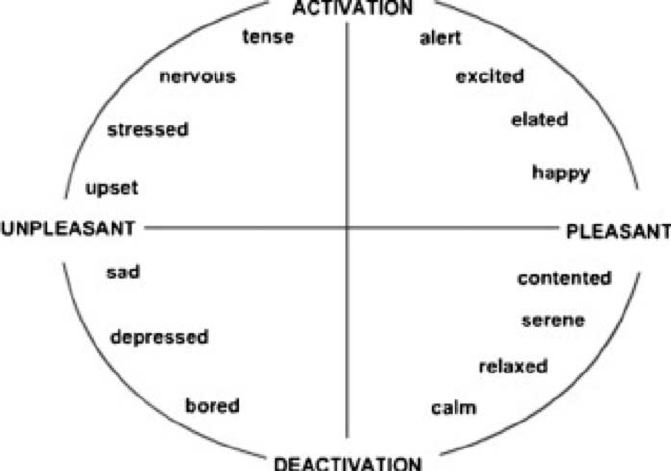
\includegraphics[scale=0.4]{images/russel_model}
	\centering
	\caption{ A. Russell�s (1980) circumplex model of affect}
	\label{fig:}
\end{figure} 

This model was later modified by Russel and Lisa Feldman Barret, which they 
described as representative of core affect, which are the most elementary 
feelings that need not be directed toward anything. Different prototypical 
emotional episodes, or clear emotions that are evoked or directed by specific 
objects, can be plotted on the circumplex, according to their levels of arousal 
and pleasure (\cite{Russell1999CoreAP}).

\paragraph{}Another model of emotion appeared in 1992. This two-dimensional 
model consists of vectors, that point in two directions. The vector model 
assumes that there is always an underlying arousal dimension and that valence 
determines the direction in which a particular emotion lies.
\begin{figure}
		\centering
		\subfloat[2D
		representation]{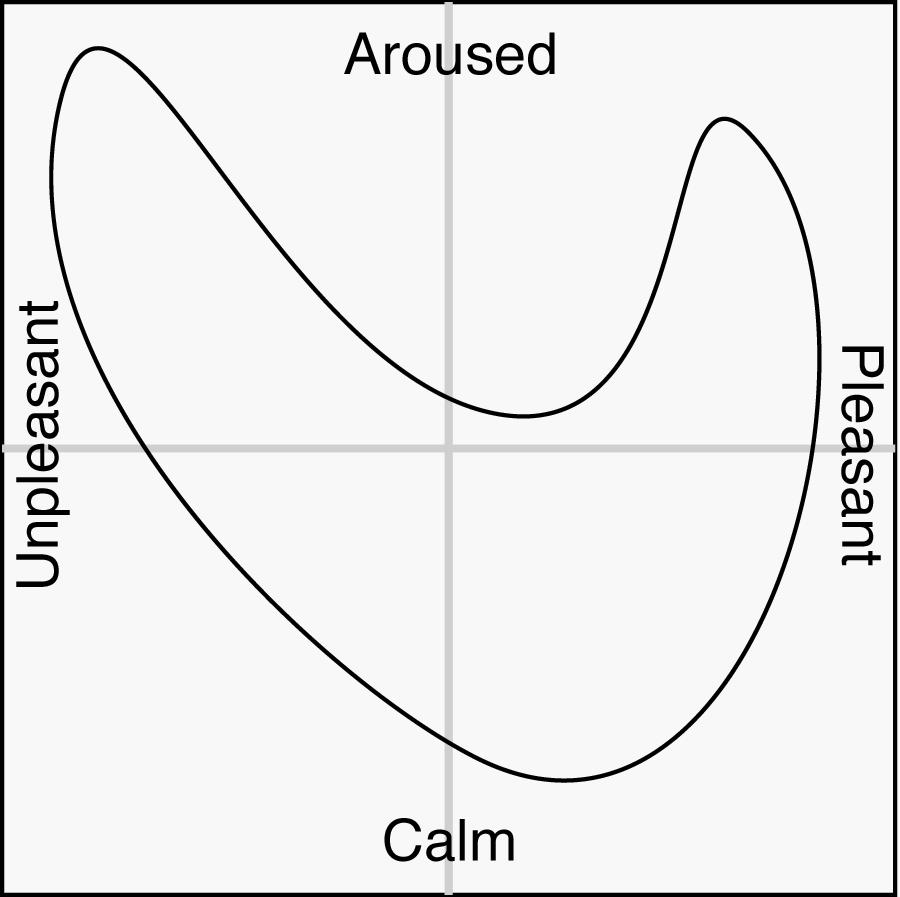
\includegraphics[width=0.2\linewidth]{images/vector0}}%
		\qquad
		\subfloat[3D 
		representation]{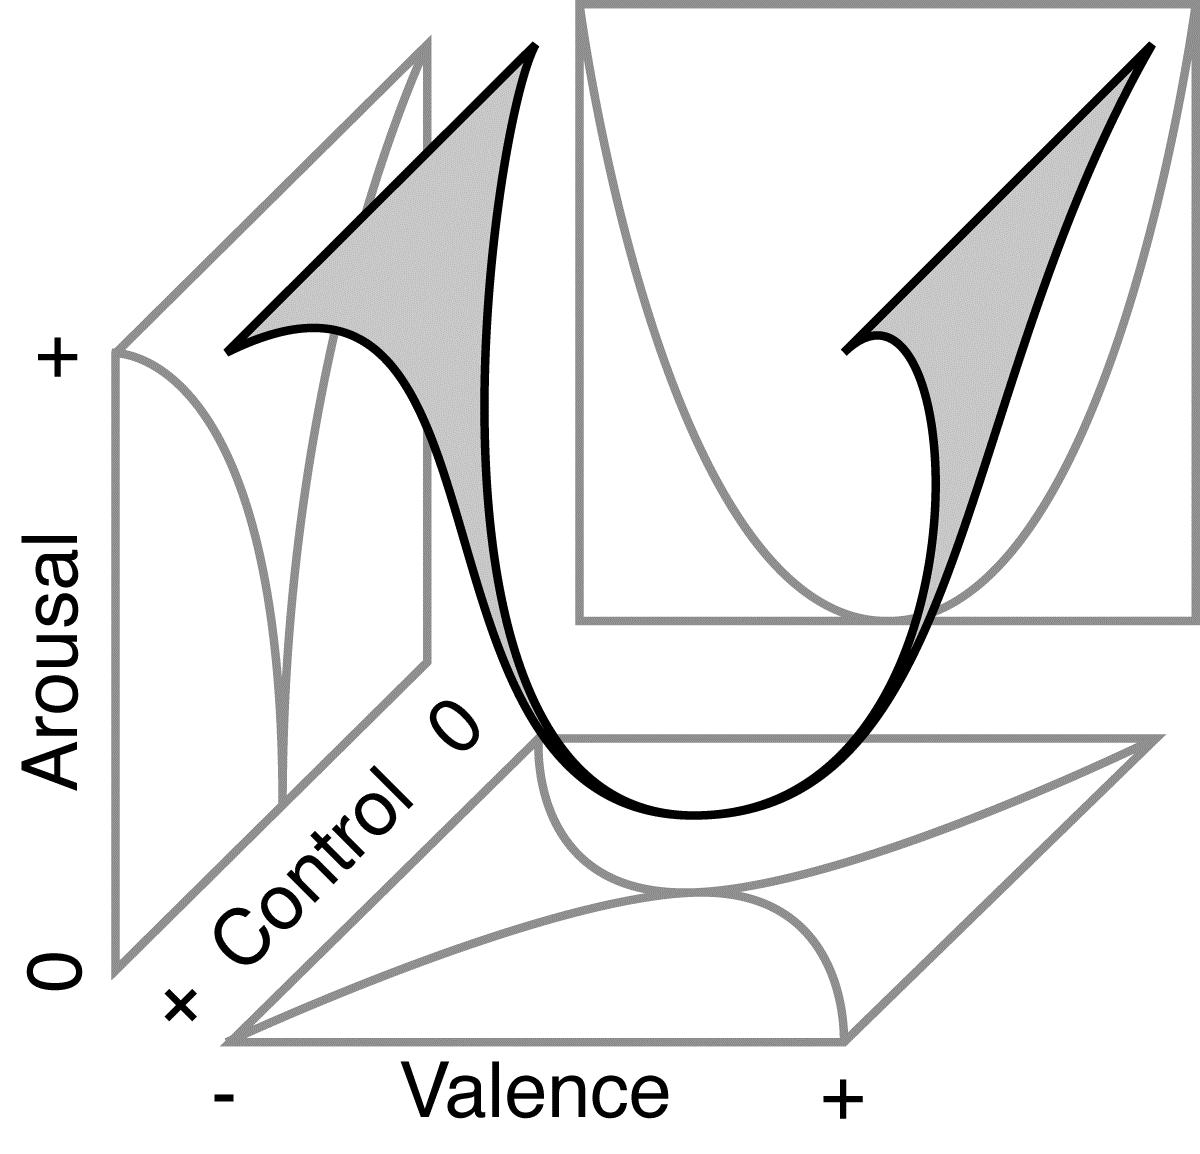
\includegraphics[width=0.2\linewidth]{images/vector1}}%
		\caption{Vector model of emotions}
		\label{fig:}
\end{figure}

\paragraph{} The positive activation � negative activation (PANA) was 
originally created in 1985 by David Watson and Auke Tellegen. It suggests that 
positive and negative affect are two separate systems. Like in the vector 
model, states of higher arousal tend to be defined by their valence and states 
of lower arousal tend to be more neutral in term of valence. In the PANA model, 
the vertical axis represents low to high positive affect and the horizontal 
axis represents low to high negative affect. The dimensions of valence and 
arousal lay at a 45-degree rotation over these axes (\cite{watson}).

\begin{figure} [ht]
	\centering
	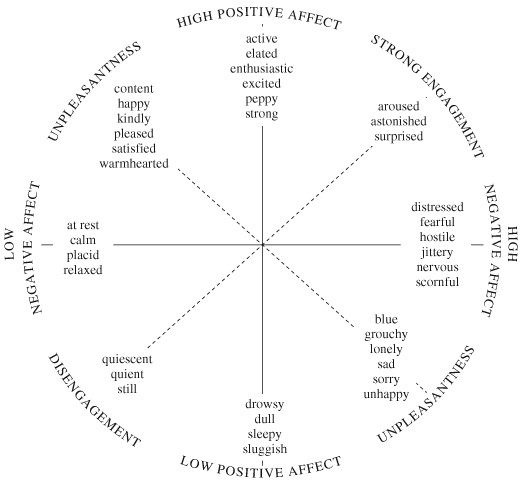
\includegraphics[scale=0.4]{images/consensual}
	\centering
	\caption{Consensual (PANA) model of emotion}
	\label{fig:}
\end{figure}

\paragraph{} In 1980, Robert Plutchik constructed a wheel of emotions. This 
model is a hybrid of both basic-complex categories and dimensional theories. 
Emotions are arranged in concentric circles, with the more basic emotions on 
the inner circles, while the outer circles are occupied by complex emotions.  
Notably, outer circles are also formed by blending the inner circle emotions. 
Plutchik suggested 8 primary contrasting pairs of emotions. Joy/sadness, 
anger/fear, trust/disgust and surprise/anticipation. Like colors, primary 
emotions can be expressed at different intensities and can mix with one another 
to form different emotions (\cite{Plutchik1988}).

\begin{figure} [ht]
	\centering
	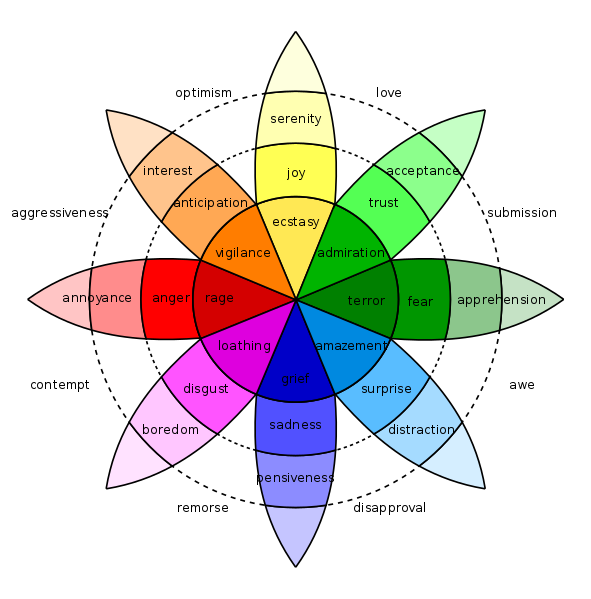
\includegraphics[scale=0.3]{images/Plutchik_wheel}
	\centering
	\caption{Plutchik's wheel of emotions}
	\label{fig:}
\end{figure}

\paragraph{} The PAD emotional state model was developed by Albert Mehrabian 
and James A. Russel. It uses three numerical dimensions, \textbf{P}leasure, 
\textbf{A}rousal, and \textbf{D}ominance to represent all emotions 
(\cite{mehrabian1980basic}). Initially it's use was in a theory of 
environmental psychology, the core idea being that physical environments 
influence people through their emotional impact (\cite{mehrabian1974approach}). 
Subsequently it was used by Peter Lang to propose a physiological theory of 
emotion (\cite{lang}). Furthermore, it was also used by Russel to develop a 
theory of emotional episodes (\cite{coreaffect}). The Pleasure-Displeasure 
Scale measures how pleasant an emotion may be. Anger and fear are, for 
instance, unpleasant emotions and thus score high on the displeasure. 
Contrarily, joy is a pleasant emotion. The Arousal-Nonarousal Scale measures 
the intensity of emotion. For instance while both anger and rage are unpleasant 
emotions, rage is much more intense than anger. Boredom, while also an 
unpleasant state, has a low arousal volume. Lastly, the 
Dominance-Submissiveness Scale shows the dominant nature of the emotion. While 
both fear and anger are unpleasant emotions, anger is dominant, but fear is a 
submissive emotion (\cite{mehrabian1980basic}).
\begin{figure} [ht]
	\centering
	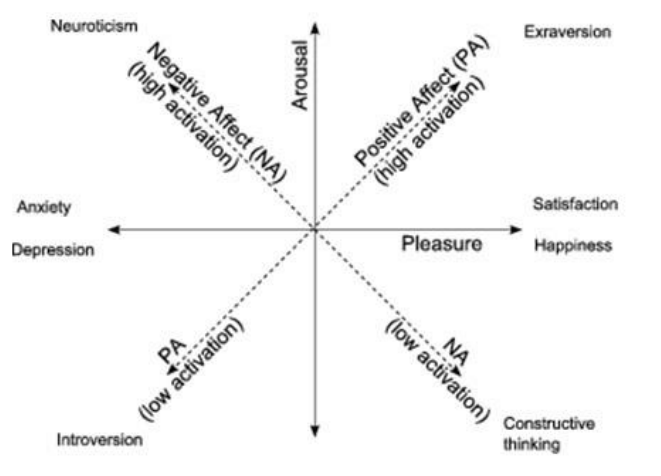
\includegraphics[scale=0.4]{images/pad_model}
	\centering
	\caption{PAD emotional state model}
	\label{fig:}
\end{figure}
A more abbreviated version of the PAD model has also been used in 
organizational studies where the emotions towards specific entities or products 
are measured. It uses just 4 values for each dimension, providing only 64 
values for emotions (\cite{abbrpad}). 

\paragraph{} An example of three-dimensional models, the L�vheim cube of 
emotion was presented where the signal substances (dopamine, noradrenaline and 
serotonin) form the axes of a coordinate system, and the eight basic emotions 
according to Tomkins are placed in the eight corners.
\begin{figure} [ht]
	\centering
	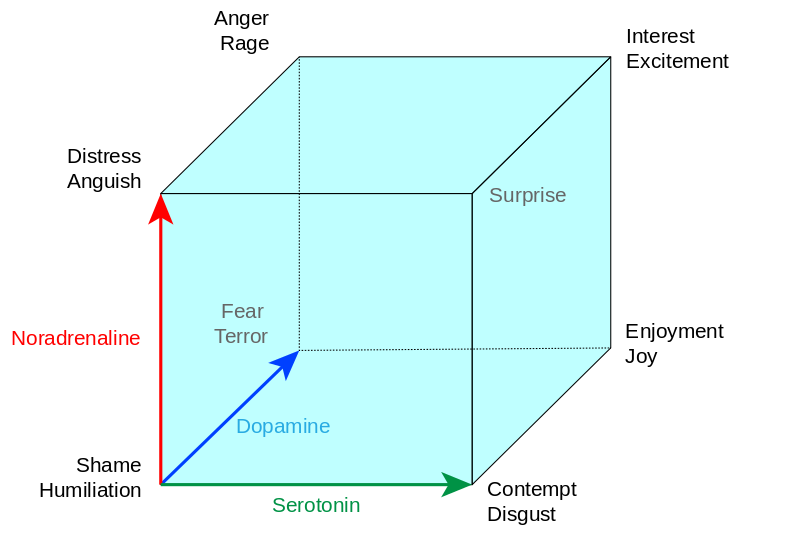
\includegraphics[scale=0.4]{images/lovheimcube}
	\centering
	\caption{L�vheim cube of emotion}
	\label{fig:}
\end{figure}
As shown on the figure below, anger is produced by the combination of low 
serotonin, high dopamine and high noradrenaline. Conversely joy is a product of 
high serotonin, high dopamine and low noradrenaline. Since none of the axis is 
identical to valence \footnote{pleasantness}, the cube seems somewhat rotated 
when 
compared to other models (\cite{Lvheim2012ANT}).


\paragraph{} Most recently Cowen and Kelter, researchers from University of 
California, Berkeley introduced a statistically derived taxonomy of emotion. 
(\cite{Cowen201702247}) \blockquote{Across self-report methods, we find that 
the [2185] 
videos [selected and shown to volunteer subjects] reliably elicit 27 distinct 
varieties of reported emotional experience. Further analyses revealed that 
categorical labels such as amusement better capture reports of subjective 
experience than commonly measured affective dimensions (e.g., valence and 
arousal). Although reported emotional experiences are represented within a 
semantic space best captured by categorical labels, the boundaries between 
categories of emotion are fuzzy rather than discrete. By analyzing the 
distribution of reported emotional states we uncover gradients of emotion�from 
anxiety to fear to horror to disgust, calmness to aesthetic appreciation to 
awe, and others�that correspond to smooth variation in affective dimensions 
such as valence and dominance. Reported emotional states occupy a complex, 
high-dimensional categorical space} 

\paragraph{}More dimensional models of emotion have been developed, though 
there are just a few that remain as the dominant models currently accepted by 
most (\cite{comparison}). There have been observed great cultural differences 
in the way in which emotions are valued, expressed and regulated. The social 
norms for emotions, like the frequency with or circumstances in which they are 
expressed also vary drastically in diverse cultures. An important piece of 
evidence that disputes the universality of emotions is language. Emotions such 
as the schadenfreude \footnote{The experience of pleasure, joy, or 
self-satisfaction that comes from learning of or witnessing the troubles, 
failures, or humiliation of another.} in German and saudade\footnote{Deep 
emotional state of nostalgic or profound melancholic longing for an absent 
something or someone that one loves.} in Portuguese are commonly expressed in 
emotions in their respective languages, but lack an English equivalent. Thus it 
is reasonable in our research to scale back on the complex, culturally 
influenced emotions and focus on the more primal, basic emotions, that may be 
more quantifiable by studying the physiological markers and responses in 
subjects.
\section{Physiological responses of emotions}
\paragraph{}When dealing with physiological effects of emotion, we come across 
a few prevalent theories. The James-Lange theory is one of the earliest 
theories of emotion within modern psychology. It was developed independently 
by 
William James and Carl Lange in 19th century. The basic premise 
\footnote{Which 
is also the point of most criticism} is that physiological arousal instigates 
the experience of emotion, i.e., the arousal precedes and causes the emotion 
(\cite{walter}). According to the Cannon-Bard theory of emotions, the emotion 
is accompanied by physiological arousal.


\paragraph{} In order for us to be able to detect and recognize emotions from 
the data samples, we need to asses which physiological effects of emotions we 
want to capture. Therefore, we need to divide our standard basic emotions 
depending on the combination of kinds and intensity of effects they have on 
human body. There is a difficulty with dealing with physiological markers of 
emotions in that not all emotions do perceivably alter the physiology of the 
subjects. That is the reason, why we need to supplement this data with the 
facial expressions or, as we have tried to confirm, ocular movements. 

\paragraph{} Anger is one of the emotions with more pronounced physiological 
signs. It comes along with faster and deeper breathing 
(\cite{respiratoryfeedback}), increased heart rate, blood pressure, 
perspiration and tensing of muscles. Fear, on the other hand, shares most of 
the surface physiological marks with anger, such as the accelerating breathing 
rate, heart rate and muscle tension, but facial expression and body language 
are vastly different. Even deeper markers, like the cortisol levels differ 
after subjecting a person to these stressors (\cite{Moons2010AngerAF}). Joy, 
sadness, disgust and surprise are similar to each other in their difficulty to 
asses using pure physiological markers and therefore requiring additional 
information, usually in form of facial expression.

\section{Current approaches in detecting and classifying emotions}
\paragraph{}As we've described motion recognition is an important object of 
studies in today's 
psychology, with many potential uses and applications. Correctly assessing and 
recognizing subject's emotion can lead to better understanding it's motivation 
and inner working. Data gained through methods described below can be used to 
assess the effectiveness of marketing, comprehensibility of lectures, usability 
of user interfaces, measure of impact of psychological therapy, etc. Previous 
implementations of emotion recognition technology often have had a multitude of 
disadvantages, which prohibited it's daily and widespread usage. Therefore, we 
have set upon creating a solution, that is modular, reasonable to wear for 
prolonged durations of time and still maintains a degree of reliability in 
captured data. We can do so by using an array of data resources, that 
complement each other, diminishing their disadvantages and reinforcing 
confidence.

\paragraph{}One particularly rich resource for data on human emotions is the 
brain. In 2015 a group of researchers in India published a paper on a system 
using EEG signals as input, Independent Component Analysis \footnote{A 
statistical procedure used for splitting up a set of mixed signals into its 
sources}, Kernel Destiny Estimation \footnote{A method used for feature 
extraction of signals by computing density estimate using kernel-smoothing 
method} and an Artificial Neural Network to  transform the inputs into 
meaningful outputs. They observed better results for clustering of EEG and ECG 
data stream (\cite{LAHANE2015574}). Similar approach was taken by researchers 
in China. Main difference in their approach is that they first applied EMD 
\footnote{Empirical Mode Decomposition} strategy to split EEG signals into a 
series of intrinsic mode functions, which were then fed as sample entropies and 
as feature vectors into SVN\footnote{Support Vector Machine} classifier for 
testing and training. With this approach, they claim to have reached accuracy 
levels of 94.98\% for binary-class tasks and  93.20\% for the multi-class task 
on DEAP database (\cite{zhang}).  Also in 2016, researchers from the Duke 
University, North Carolina demonstrated an emotional recognition technique 
using functional MRI with results, that brain-based models may, in future, 
allow us deeper understanding and assessing emotional status in clinical 
settings, particularly in individuals incapable of providing self-report of 
their own emotional experience (\cite{kragel}). These techniques are, however, 
impossible to replicate on greater scale and in the context of a classroom, or 
other commonplace environment.

\paragraph{}Another indicator of the subject's emotional state is heartbeat. 
Research published in May 2013 in International Journal of Engineering Trends 
and Technology shown compelling data gathering by means of 
ECG\footnote{Electrocardiography} and shown 
differences in ECG signal in subjects in chosen emotional states. 
\footnote{This study was limited to joy, sadness, fear and anger} 
(\cite{shalini2013emotion}). More complex approach was taken by researchers at 
University of Calabria in collaboration with Washington State University. 
Instead of applying a single or a few sensors to study physiological states, 
they used a whole BSN\footnote{Body Sensor Network, specialized Wireless Sensor 
Network applied to the whole human body.} Such networks can include 
accelerometers, gyroscopes, pressure sensors for body movements
and applied forces, skin/chest electrodes (for electrocardiogram
(ECG), electromyogram (EMG), galvanic skin response (GSR), and
electrical impedance plethysmography (EIP)), (PPG) sensors, microphones (for 
voice, ambient, and heart sounds), scalp-placed electrodes for 
electroencephalogram (EEG) (\cite{gravina}). Albeit they were not focusing 
primarily on emotion recognition, this survey shows consequential advancement 
in the state-of-the-art body data collection, especially in the data fusion 
techniques. Similar approach using a variety of sensors and data sources was 
also taken by \cite{MOSCIANO201748} to reasonably accurately classify the two 
dimensions of affect both normal and simulated critical working conditions.

\paragraph{}An interesting approach to emotion detection and classification is 
based upon speech patterns and variations and are better suited for emotions, 
which are otherwise hard to physiologically measure, such as sadness and joy. 
One study shows, that speech signal and feature distances of letters and words 
vary depending on the mood and emotional state of the subject. The study was 
done upon the sample size of 30 people, however, researchers point out, that 
for getting better accuracy, one should consider the data collected from one 
person rather than considering the data from a group of people 
(\cite{DAVLETCHAROVA201591}).

\paragraph{}In terms of evaluating arousal, respiration-based emotion 
recognition shows promise. A study in China showed, that using respiration data 
to evaluate valence and arousal levels of Russel theory, they reached 
classification accuracy of valence and arousal at 73.06\% and 80.78\%, 
respectively (\cite{zhang2}). When compared to other studies using ECG or 
EEG data, the accuracy of valence levels are not exceptional, however the 
classification accuracy of arousal better than most other approaches.

\paragraph{}A study on thermal behavior of anger, disgust, fear, joy and 
sadness was carried out in 2016. When an emotion occurs a change in facial 
temperature appears due to the blood flow that the body emits through blood
vessels in the subcutaneous area (\cite{stephanos}). For example, research 
focused on the emotion of joy, in other words, when a subject is smiling, it has
been found that the temperature of the nose and forehead
decreases during this event (\cite{SALAZARLOPEZ2015149}). Biomedical thermal 
images of the facial
expressions of 44 subjects were captured experiencing the five studied 
emotions, with results of this test at 89.9\% success rate (\cite{Albarran}).

\paragraph{}Another novel approach was experimented with by researchers from 
American University of Sharjah, United Arab Emirates. They have created a 
software touch keyboard, that was installed on Android smartphones, which then 
have been collecting sensor data while users were typing on the keyboard. As 
they have been typing, he or she were prompted to indicate their current 
emotional state, which then tagged the sensor data collected for the particular 
user. Afterwards the data was classified by multiple machine learning 
algorithms to find the best classification method. Based on 
ROC\footnote{Receiver Operating Characteristic} and Precision-Recall curves, it 
was concluded that both J48 and Multi-response linear regression performed
well. This system demonstrates that it is possible to enable emotion 
recognition on mobile phones using built-in sensors (\cite{ZUALKERNAN20171}). 
More research is, nevertheless, needed to precisely ascertain the accuracy and 
applicability of such solution in common practice.

\paragraph{}One approach seems to be very promising, especially due to it's 
implementation in commercial solutions and services. That approach is based on 
facial expression evaluation and it is used by a wide variety of software 
vendors and research institutions. One such research has used Microsoft Kinect 
for 3D face modeling with a goal to computationally recognize facial 
expressions of seven basic emotional states: neutral, joy, surprise, anger, 
sadness, fear and disgust. The subjects of the experiment were six men aged 
26-50 years, told to mimic expressions shown on the screen. Researchers  used 
nearest neighbor classifier (3-NN) and two-layer neural network classifier (MLP)
with 7 neurons in the hidden layer with output accuracy rate of 96\% for 
random division of data and 73\% for "natural" division of data 
(\cite{TARNOWSKI20171175}).
%mention affectiva and other commercial sdk and api

\paragraph{}Last but not least, one of the more recent\footnote{And less 
explored.} approaches taken in affective computing is gaze and pupil tracking. 
This builds on classic theories (\cite{hess} ; \cite{beatty}) and tries to 
implement eye-tracking techniques to investigate emotional state and behavior 
of subjects. They were successful in distinguishing between emotions, albeit 
having to limit them from the core seven to four. Accuracy of their recognition 
ranged in the interval from 80 to 90\% (\cite{maskeliunas})

\paragraph{}There are two questions, that remains unanswered. Is our current 
method of selecting impulses the correct one? Are we rating approaches the 
right way? In research mentioned above, there are mainly two types of 
referential data. One is based on self-identifying emotions, the other on using 
previously assorted categories of pictures or impulses. As we've mentioned 
before, self-identifying emotions is a hard task for most people and it is the 
task, that we aim to solve. Also, is the methodology we use, to personally 
evaluate emotions the correct one? We usually refer to the previous 
evaluations, that trace back to psychologist and we take their emotion 
assessments at face value. It might be wise, that we should ignore previous 
results and rather try to classify and categorize emotions from ground up and 
later compare them with historical data. Finally, most of the researches 
delving into face expression-based emotion recognition declare their statistics 
based upon the success rate of recognizing simple expressions, not emotions 
themselves.

\subsection{Emotion recognition used in commercial environment}
\paragraph{}With plethora of possible applications and use-cases, from 
marketing, automotive industry, health care, education and psychology research, 
it is no wonder that a lot of industries are pushing towards better and faster 
classification of emotions. Consequently the number of dependable 
SDK\footnote{Software development kit -  A set of software development tools 
that allows the creation of application for a certain software package, 
framework, hardware platform, etc.} and API\footnote{Application programming 
interface - A set of functions and procedures that allow the creation of 
applications which access the features or data of an operating system, 
application, or other service.} grows rapidly. A few of them also merge and/or 
work together towards better integration.

\paragraph{}Emotient was one such company. Their FACET SDK allows application  
to track and analyze the emotional responses of users in real-time, detecting 
and tracking expressions of primary emotion, as well as overall positive, 
negative and neutral sentiments and blended composites of two or more emotions. 
In 2013 they partnered with iMotions to provide a facial expression 
recognition, EEG and GSR analysis platform to Procter and Gamble, the United 
States Air Force and Yale University. As part of the agreement between the two 
companies, Emotient's industry-leading emotion recognition solution was fully 
integrated into iMotions Attention Tool, an eye tracking and biosensor software 
platform for research and usability. In 2016 Emotient got acquired by Apple and 
their website is no longer online.

\paragraph{}Next in consideration was Eyeris EmoVu. It's a closed-source, 
multi-platform SDK and API, that supports all three major desktop operating 
systems: Microsoft Windows, macOS and GNU/Linux. It has language hooks for C++, 
Java, VB.NET, Python, Objective-C, Node.js and more. Their pricing starts with 
a free license, that covers the analysis of 500 frames per month. It's declared 
features are \begin{multicols}{2}
	\begin{itemize}
		\item Emotion Recognition
		\item Gender Recognition,
		\item Age Recognition\footnote{Although not in numerical values, but in 
		labels such as Child, Young Adult, Adult and Senior},
		\item Face Recognition,
		\item Facial Tracker,
		\item Engagement and Mood metrics.
	\end{itemize}
\end{multicols}

EmoVu's main drawback is lack of clear information about the SDK availability, 
since they only mention it on their website in unclear terms and the pricing 
only mentions API.

\paragraph{}An interesting approach to confronting racial bias in face 
recognition algorithms is shown by Kairos. As several studies shown, there is a 
great difference between the error rates in human races.  The extent of these 
biases are reflected in an error rate of 0.8 percent for light-skinned men, and 
as high as 34.7\% for dark-skinned women. Since this problem can have very far 
reaching implications, it's important to try to mitigate it. The solution 
advocated by Kairos is to: \begin{enumerate}
	\item Trust the process - as it's a new technology with room to grow,
	\item Improve the data sets - gathering, training, and testing data from a 
	population that is truly representative of global diversity
	\item Seek constant feedback - trying to see what the users and communities 
	see.
\end{enumerate} (\cite{kairos})

\paragraph{}Microsoft, the epitome of a immense corporation, has entered this 
technological race with the launch of their Project Oxford. It's a collection 
of artificial intelligence APIs with focus on computer vision, speech and 
language analysis. It got it's own fair share of controversy with it's mediocre 
launch, but continued to improve steadily. Project Oxford's tools enable face 
detection and emotion detection \footnote{It uses a model of core seven 
emotions plus neutral.} Unfortunately, the API works only with photos. The 
pricing start with a free plan, that covers 30,000 transactions per month.

\paragraph{}InSight SDK is facial recognition C++ toolbox developed by 
Sightcorp in collaboration with the University of Amsterdam. It boasts a large 
set of features, apart from face detection and emotion recognition, it uncovers 
gaze estimation, head pose estimation and motion tracking features. InSight 
does not provide academic trials, therefore we could not evaluate their 
performance.



\paragraph{}Another company that partnered with iMotions is Affectiva. The deal 
came with Affectiva making their Affdex facial coding and emotion analytics 
software available on the iMotions Biometric Research Platform. With this joint 
solution human behavior researchers can combine facial coding and emotion 
analytics with eye tracking, brainwave measurement (EEG), as well as 
physiological sensors (GSR, ECG, EMG) on top of traditional surveys and 
questionnaires, which are also fully integrated. The main Affectiva's 
achievement was the amassment of the world's largest emotion data repository. 
By 2018, they analyzed over 6 million faces from 87 countries The offer both 
API \footnote{Which can be used online on a thin client.} and SDK {Which allows 
applications to run locally and without needing Internet connection.} for the 
major platform like Android, iOS, GNU/Linux, Windows and macOS. They have built 
their massive data set of facial expressions by analyzing millions of face 
videos, of people engaged in various activities, such as watching media 
content\footnote{i.e, ads, movie trailers, television shows and online viral 
campaigns}, driving cars, people in conversational interactions and animated 
gifs\footnote{Via the partnership with giphy}. To get this impressive amount of 
data, Affectiva partnered with their market research partners such as Millward 
Brown, Unruly, Lightspeed, Added Value, Voxpopme and LRW and also with partners 
in the automotive industry, robotics and Human Resources space. Affectiva's 
Affdex SDK was tested on 10 000 images to verify the generalizability of 
algorithms. Those images cover different lightning conditions, both genders, 
various poses of participants, etc. Via the SDK, application can access and 
read multiple metrics. Those include 7 emotion metrics, 20 facial expression 
metrics, 13 emojis and 4 appearance metrics. Apart from the 7 emotional states, 
the SDK surfaces also the Engagement\footnote{A measure of facial muscle 
activation that illustrates the subject�s expressiveness. The range of values 
is from 0 to 100.} and Valence \footnote{A measure of the positive or negative 
nature of the recorded person�s experience. The range of values is from -100 to 
100.} metric. The SDK offers four main features. \begin{enumerate}
	\item Face and facial landmark detection,
	\item Face texture feature extraction,
	\item Facial action classification,
	\item Emotion expression modelling.
\end{enumerate} (\cite{affdex}) The SDK are offered under various licensing 
deals, with a free Commercial Evaluation License valid for 60 days, or Student 
Evaluation License valid for 6 months. The API is paid by the processing time, 
with pricing starting at \$1/minute of video processed. Affectiva's mapping of 
expressions onto emotions builds on EMFACS mapping, developed by Friesen and 
Ekman. EMFACS is a variant of FACS system, that considers only emotion-related 
facial actions. (\cite{ekman1997face})
The table \ref{table:1} shows the relationship between the facial expressions 
and the emotions predictors as used in the Affdex SDK.

\begin{table}[h!]
	\centering
	\begin{tabular}{||c | c | c||} 
		\hline
		\hline
		Emotion & Increase Likelihood &  Decrease Likelihood \\ [0.5ex] 
		\hline\hline
		Joy & Smile & Brow Raise, Brow Furrow  \\ 
		\hline
		Anger & Brow furrow, Lid Tighten, & Inner Brow Raise,  \\ 
		& Eye Widen, Chin Raise, & Brow Raise,  \\ 
		&  Mouth Open, Lip Suck & Smile  \\
		\hline
		Disgust & Nose Wrinkle, Upper Lip Raise & Lip Suck, Smile  \\
		\hline
		Surprise & Inner Brow Raise, Brow Raise & Brow Furrow \\
		 & Eye Widen, Jaw Drop & \\
		 \hline
		Fear & Inner Brow Raise, Brow Furrow & Brow Raise, Lip Corner 
		Depressor  \\ 
		& Eye Widen, Lip Stretch & Jaw Drop	Smile \\
		\hline
		Sadness & Inner Brow Raise, Brow Furrow & Brow Raise, Eye Widen, Lip 
		Press  \\ 
		& Lip Corner Depressor & Mouth Open, Lip Suck, Smile \\
		\hline
		Contempt & Brow Furrow, Smirk & Smile  \\ [1ex] 
		\hline
		\hline
	\end{tabular}
	\caption{Relationship between the facial expressions and the emotions 
	predictors}
	\label{table:1}
\end{table}

\begin{table}[h!]
	\centering
	\begin{tabular}{||c | c||} 
		\hline
		\hline
		Increase Positive Valence Likelihood & Increase Negative Valence 
		Likelihood 	\\ [0.5ex] 
		\hline
		\hline
		 Smile & Inner Brow Raise   \\ 
		
		Cheek Raise & Brow Furrow   \\ 
		
		 & Nose Wrinkle  \\
		
		 & Upper Lip Raise  \\
		
		 & Lip Corner Depressor  \\ 
	
		 & Chin Raise   \\ 
		
		 & Lip Press   \\ 
		 & Lip Suck  \\ [1ex] 
		\hline
		\hline
	\end{tabular}
	\caption{Markers increasing and decreasing predicted valence metric. 
	likelihood.}
	\label{table:2}
\end{table}

Lastly, the engagement of the subject is measured as a weighted sum of the 
following facial expressions:
\begin{multicols}{2}
\begin{itemize}
	\item Brow raise,
	\item Brow furrow,
	\item Nose wrinkle,
	\item Lip corner depressor,
	\item Chin raise,
	\item Lip pucker,
	\item Lip press,
	\item Mouth open,
	\item Lip suck,
	\item Smile.
\end{itemize}
\end{multicols}

\paragraph{}Due to the ease of use, clear documentation, offline capabilities 
and free 6 month trial, we have decided to proceed using Affectiva's Affdex SDK.


\chapter{Data gathering methodology}
\paragraph{}As we've demonstrated, there are great many approaches to take and 
physiological markers to explore. Due to the nature of our desired use-case, 
we've decided to omit those physiological signs and pertaining sensors, that 
would excessively constrain and disturb the user. Similarly, we did not employ 
techniques, that would restrict our application from workplace or school 
environment. Therefore, we did not use EEG, fMRI scanning, neither Thermal 
imagining, nor speech recognition. For our body sensors, we have chosen a 
simple, inexpensive optical heart rate sensor, GSR\footnote{Galvanic Skin 
Response} sensor and Arduino to read and resend collected data. Furthermore, we 
used a headset with two high-speed infrared cameras with infrared illumination 
and one 1920x1080 "world" camera. To provide referential emotion values, we 
used a regular 720p web camera, and processed the camera feed with modified 
Affdex sample OpenCV application.
\section{Hardware}
\paragraph{}The research has been done using two different computers. 
\begin{itemize}
	\item Desktop workstation with hexa-core AMD FX-6300 clocked at 4.0GHz, 
	8GB of RAM and Radeon 7700 GPU,
	\item Laptop with quad-core Intel Core i7-4770HQ, 16 GB of RAM and NVidia 
	860M GPU.
\end{itemize}
\paragraph{}These two computers proved able to fully satisfy hardware needs of 
the 
research. We have also tried to run the modifiet Affdex sample application on 
Raspberry Pi 3B with official IR camera, however we found out, that the single 
board computer was greatly lacking computing power and would freeze, hang and 
drop frames with even one face detected on video feed. Powerful hardware was 
needed not only for the use of Affectiva SDK, but also for the Pupil Capture 
software, supplied by the manufacturer of our headset. These two applications 
taxed both our computers close to peak load, although since our EmoSens data 
collection application requires very few resources, it did not negatively 
impact our experiments.

\paragraph{}The heart rate data was gathered by Pulse Sensor Amped SEN-11574, a 
plug-and-play heart rate sensor for Arduino and Raspberry Pi. It's a simple, 
inexpensive optical sensor, that incorporates amplification and noise 
cancellation circuitry on a single board. We did find out, that it requires 
tight strapping to subject's skin, otherwise the data collected has been 
inconsistent with reality.
\begin{figure} [ht]
	\centering
	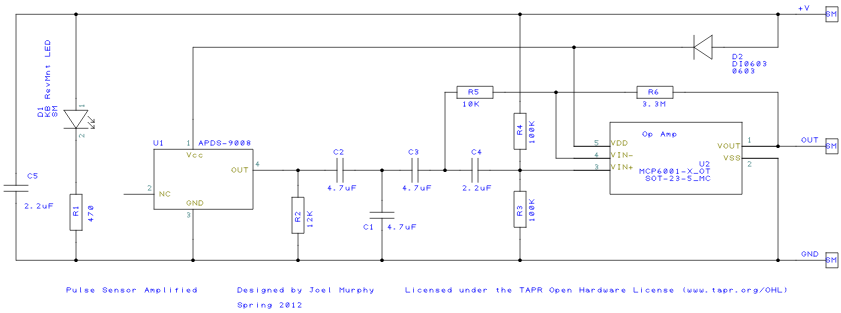
\includegraphics[scale=0.5]{images/HRCircuit}
	\centering
	\caption{Pulse Sensor Amped SEN-11574 circuitry}
	\label{fig:}
\end{figure}
\newpage

\paragraph{}The Galvanic Skin Response data was collected using Groove GSR 
sensor. Groove is an Arduino shield maker, with a plethora of different sensors 
available to buy. Since we only needed GSR and it is a relatively trivial task 
to wire the Sensor directly to Arduino while circumventing the need for the 
Groove shield itself, we connected the Groove GSR sensor straight to Arduino's 
GPIO pins.

\begin{figure} [ht]
	\centering
	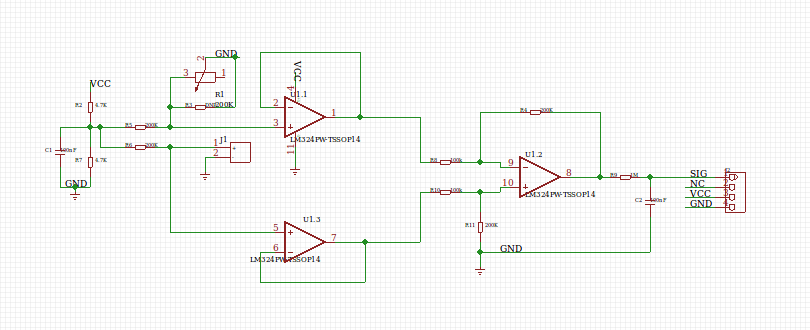
\includegraphics[scale=0.5]{images/GSRCircuit}
	\centering
	\caption{Groove GSR Sensor circuitry}
	\label{fig:}
\end{figure}

\begin{figure}
	\centering
	\subfloat[Pulse Sensor Amped 
	SEN-11574]{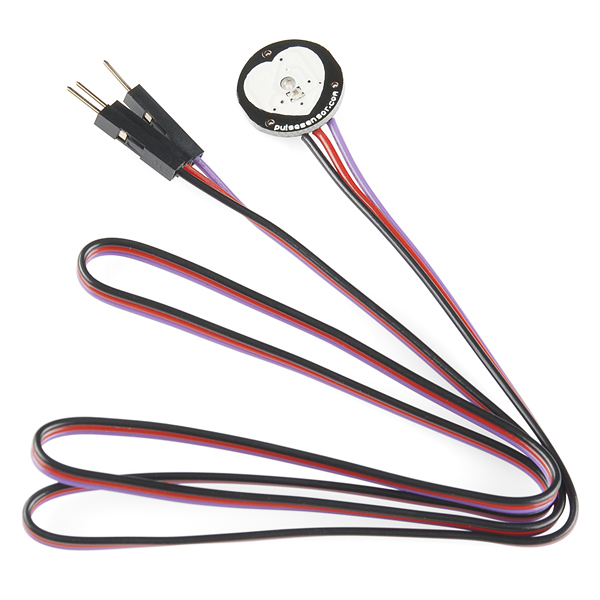
\includegraphics[width=0.2\linewidth]{images/HRSensor}}%
	\qquad
	\subfloat[Groove GSR 
	Sensor]{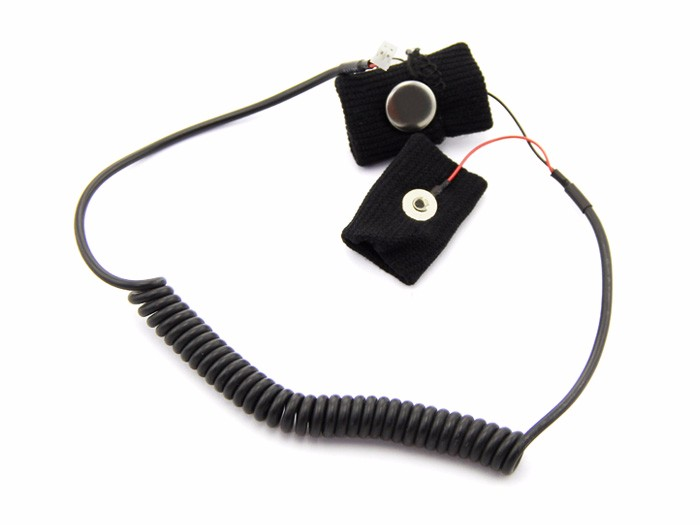
\includegraphics[width=0.25\linewidth]{images/GSRSensor}}%
	\caption{Sensors}
	\label{fig:}
\end{figure}

\paragraph{}Both of these sensors were sewn into a fingerless glove and wired 
to Arduino Due connected via USB cable to computer.

%add schema of the arduino wiring

\newpage

\paragraph{}The Pupil headset consists of two high-speed 200Hz IR eye cameras 
with illumination and a single FullHD World camera connected together to a 
computer using USB-A to USB-C connector.
\begin{figure} [ht]
	\centering
	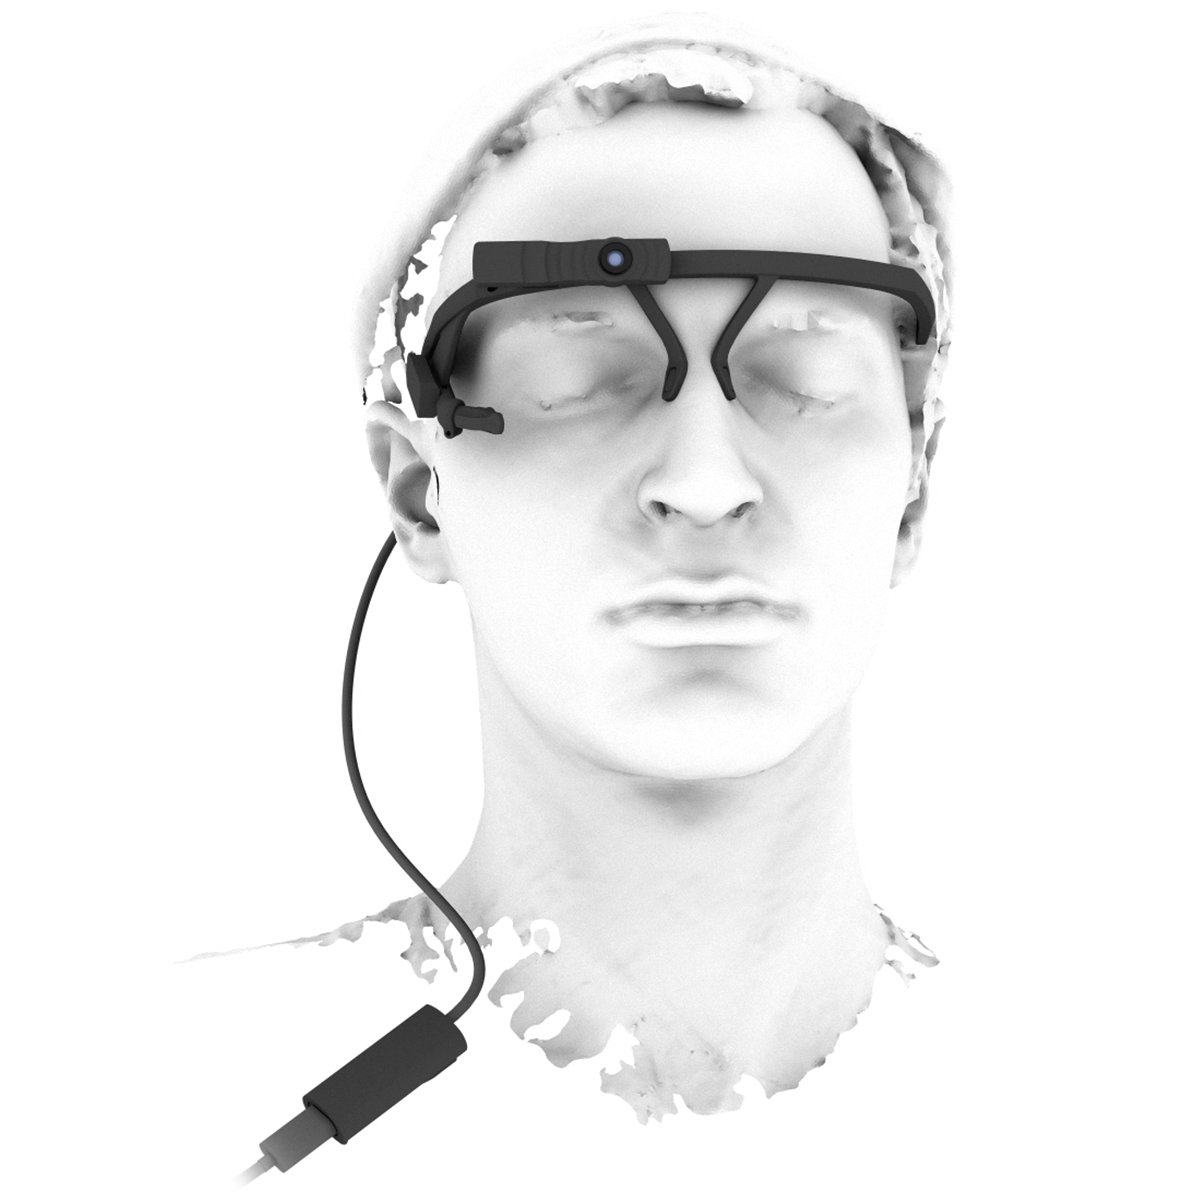
\includegraphics[scale=0.2]{images/pupil}
	\centering
	\caption{Pupil headset}
	\label{fig:}
\end{figure}

\section{Software}
\paragraph{}Both development and experiments took place on computers running 
Ubuntu 16.04. 
We have chosen this operating system, as it has large community of developers, 
computer scientists and because most innovative frameworks and SDKs target this 
platform. To create the data collection software, we have used the Qt5 
application framework. It's main advantages in our use-case is it's 
intuitiveness, open-source and cross-platform compatibility. It has bindings 
with Python\footnote{PyQt} and C++. It also adds extensions to C++, including 
signals and slots, which greatly simplify handling of events, thus helping in 
development of GUI. It was compiled by GNU GCC 5.4.0. The Arduino is 
programmable in a it's own variant of simplified C++, that forgoes features of 
the language such as inheritance. Last but not least, the modified Affdex 
webcam application is written in C++, albeit due to the incompatibilities with 
newer compilers was compiled in GNU GCC 4.8.

\paragraph{}This leads us to the unexpected setback that we came across. Both 
Affectiva and Pupil use OpenCV 2.4, but Affectiva forked it's version and when 
building with CMake on a recent operating system, it will either fail, or 
overwrite shared libraries, thus breaking QT5 and Pupil. One solution to this 
problem might be to install Affectiva sample application on a separate 
computer, but since we aimed to create a compact solution, we opted for 
installing it in a virtual machine running stock Ubuntu 16.04 with only the 
libraries, that Affectiva requires and nothing else.

\paragraph{}Since Affectiva's licence agreement prohibits it's integration with 
a copyleft open source licensed projects \footnote{In our case GNU GPL v2} we 
have modified the sample OpenCV application to send out data serialized in 
messagepack over zeromq, thus eliminating the need to include it in our 
project. This has added benefit in that our project is therefore modular and 
can use any and all face or other emotion recognition SDK with 
little to no changes to our source code.

\paragraph{}ZeroMQ is a large community of projects with focus on decentralized 
messaging and computing engines. Both software and protocols are open source 
and maintained by community of experts. The original core engine is libzmq, 
available in repositories of most GNU/Linux distributions, but also available 
to install on all the other major operating systems. On top of libzmq, there is 
a large number of language bindings, such as PyZMQ, CZMQ, CPPZMQ, NZMQT 
\footnote{Our project uses NZMQT due to it's great integration with QT5's 
signals and slots}. There are also native languages written for Java, .NET, 
JavaScript and many others. Most importantly, it's really lightweight and fast. 
The core library is only 20K lines of C++ code and the message throughput is 8 
million messages per second with latency in microseconds. There are three main 
patterns used in ZeroMQ. Request-Reply, Publish-Subscribe and Pipeline pattern. 
(\cite{hintjens2013zeromq} ; \cite{Akgul})
 

\paragraph{}MessagePack is a low-overhead binary serialization format. Compared 
to the better know binary serialization format BSON, it's better in every 
possible technical aspect. It's faster, smaller, and even more compatible to 
JSON than BSON is. It's got support for dozens of languages, notably for 
Python, Java, C, C\# and multiple standards of C++. MessagePack by design 
solves 
the problem of interprocess communication, especially if the processes are 
written in different languages, or are even running on different platforms.

\paragraph{}For our project, we opted to use the Publish-Subscribe pattern, 
with Pupil Capture and Affectiva being the Publishers and our application 
serving as a Subscriber to their messages serialized with MessagePack. That way 
we ensure, that the communication is fast and reliable and also that the 
peculiarities of different programming languages are covered for ease of use. 

\begin{figure} [ht]
	\centering
	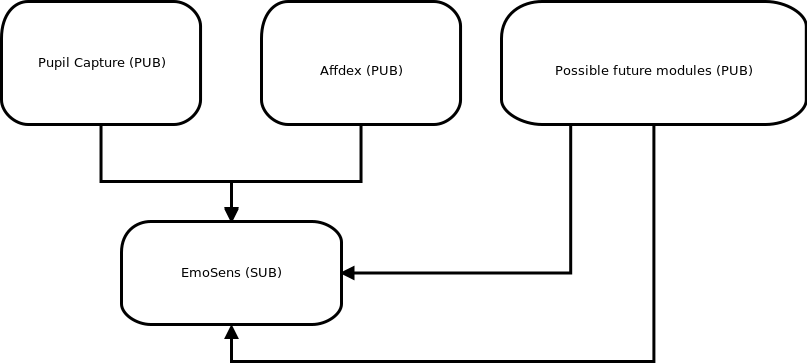
\includegraphics[scale=0.4]{images/zeromqdia}
	\centering
	\caption{Simplified diagram of the data flow.}
	\label{fig:}
\end{figure}

\paragraph{}For visualization of collected data, we have used two QT libraries. 
The QtCharts library, which is included in the open-source Qt 5.10 
installation, and also the QCustomPlot for more complex and granular control. 
QCustomPlot is a free and open-source Qt C++ widget for plotting and data 
visualization. It has no dependencies and is well documented. It even supports 
exporting to various format such as vectorized PDF files and rasterized 
pictures in PNG, JPG and BMP.

\section{EmoSens application}

%TODO: add description of the classes, screenshots of the gui, etc.

\section{The experiments}

%TODO : Add the description of the data collection process, pictures, etc.

\chapter{Data evaluation}

%TODO: Evaluate the data from the visualization and maybe nerualt network

\chapter{Results}

\chapter{Discussion}
\printbibliography
\end{document}